\chapter{Methodology}
\label{chap:methodology}

\section{Measurement Process}

The time series used in this work represent network end-to-end measures of a
cable-television infrastructure, which runs DOCSIS with asymmetric download and
upload bandwidths. Home routers connected to the cable modem communicate with
one or more servers strategically located by the ISP\@. Measurements results
from
each home router are consolidated every half hour and, by the end of every day,
are transferred to a database. The software responsible for these procedures was
developed by TGR (a startup at COPPE/UFRJ) in collaboration with the university
(UFRJ), and is spread over a customers subset of a major Brazilian ISP\@.

In~\cite{a_preliminary_performance_measurement_study_of_residential_broadband_services_in_brazil},
a preliminary investigation of several metrics is presented. To measure the
round
trip packet loss fraction and RTT between the home router and the associated
server, the
home router sends a train of short UDP packets, and then the server bounces back
them. The data here presented considers a train of 100 UDP packets of 32 bytes,
separated by 1 millisecond. This dissertation only deals with these two
metrics.

The resulted time series are unevenly spaced due to a range of reasons. First,
measurements are initiated only if the residential link is not under use by the
ISP customer. Also, the client may have no Internet connection to start a
measurement, or even be without electrical energy.

Each server is responsible to conduct measurements of several end-users.

The traceroute is implemented through UDP packets, since this type of packets
is more accepted in the Tier-2 and Tier-3 ISP's of the environment.

\section{Pipeline}

This section describes, in a high level abstraction, the proposed workflow
used to detect network events and localize their cause. When necessary, some
steps are better explored in further sections.
The analysis seeks for events during a specific time period, in a single
measurement server, and considers a
single metric (loss fraction or RTT), which are specified as parameters.
Therefore the complete analysis, considere several executions, for different
servers, and parameters.
Figure~\ref{fig:pipeline} illustrates the process.

\begin{figure}[H]
    \centering
    \includegraphics[width=0.9\linewidth]{./figures/methodology/pipeline/pipeline.png}
    \caption{Pipeline.}
\label{fig:pipeline}
\end{figure}%

The workflow starts with the End-Users Filtering step,
which aims to remove clients that can negatively affect the analysis.
As an example, this work eliminates clients
that don't have enough measurements, or present
traceroute inconsistencies (in Section~\ref{sec:spatial_correlation}
this issue is better explored).

The Change Point Detection phase preprocess the end-users time series and
identify change points.
Also, the change points are classified in three types of events: failure,
improvement, or inconclusive. For both metrics, a change point defines a
failure event if the average of the window after this point is greater than the
average of the window before. The improvement event is analogous, however is
identified by a mean decrease.
The inconclusive event means that the segments averages are too close.

The Spatial Correlation procedure cluster the end-users in end-groups
according with their location in the network.
This stage must produce a specific grouping structure, which is detailed in
Section~\ref{sec:spatial_correlation}.

The Events Times Correlation aims to combine similar events of different
end-users of an end-group. For example, if three end-users detect a failure at
the same time, this information will be identified in this step. The resulted
grouped events are then named as network events.
The details of this method are clarified in
Section~\ref{sec:events_times_correlation}.

Finally, to localize the events cause, the Spatial-Time Correlation
correlates network events
from different user-groups with the end-groups structure.
This is better exaplained in Section~\ref{sec:spatial_time_correlation}.

\section{Spatial Correlation}
\label{sec:spatial_correlation}

This procedure aims at cluster end-users in user-groups.
An end-user can
participate in more than one end-group.
In each user-groups the end-users of this group share at least one physical
equipment.
To reasons that will be explained in
Session~\ref{sec:spatial_time_correlation} the resulting end-groups structure
must be a tree.

The end-users are clients of a Tier-3 ISP\@. The measurement server localization
is classified in two cases. In the OFF-NET case, the traffic between the
end-user and server goes through a Tier-2 ISP\@. In the ON-NET case, the traffic
between them doesn't leave the Tier-3 ISP infrastructure. The Tier-3 doesn't
applies load balancing and don't have MPLS, however the Tier-2 ISP is more
complicated, presenting both techniques. The IP topology is reconstructed
through traceroute measurements started from the end-users to the server. As
with the other metrics, the traceroute is executed in every 30 minutes.

Therefore fixing a single server, and only the ON-NET case, the lack of load
balancing gurantee that the traceroute
reconstruction topology lead to tree structure. In this case, each router that
responds the traceroute can be used as an user-group. In this context the leafs
are the first routers that appear in the traceroute, and the root is the
server. The internal vertexes are routers from the Tier-3 ISP\@.

In HFC network, the first network component to respond to the traceroute can be
a CMTS, however some CMTSs are configured to not answer ICMP packets. However,
since the end-user and the associated CMTS are in the same subnetwork, the CMTS
respond with it's private IP, that can be used by different CMTS\@. Therefore to
differentiate distinct CMTS that have the same private IP, each vertex of the
topology is defined by the IP responded + the first public IP that appears to
the path to the server.

However inn the OFF-NET case the traceroute reconstruction don't lead to a
tree due to the load balancing. To overcome this problem the vertex associated
with the Tier-2 ISP is compressed to only one vertex. In only one case this
procedure don't lead to a tree, when the traffic from the Tier-2 ISP to the
Tier-2 ISP can leave to different routers. By now this case was removed from
the analysis.

In Figure~\ref{fig:} contains an example of the reconstructed
topology. The names and IPS were aninymazed.

Also, in End-Users Filtering, some clients are removed due to traceroute
inconsistencies~\cite{avoiding_traceroute_anomalies_with_paris_traceroute},
such as the same node that appears more than once in different
hops, traceroutes that don't reach the target.

\section{Events Times Correlation}
\label{sec:events_times_correlation}

The motivation of this step is to, given the change points of each end-user of
an end-group, infer information of network events that can be common to these
end-users.

There are two main reasons to detect the same network event, such as an
equipment failure, at different times in different clients. The first one is
related to the fact that the time series are not regularly sampled. The second
one is due to the change point detection algorithm behavior.
Therefore, a procedure to group end-users events based on their type and time,
should be flexible enough to take into consideration time delay effects, and
the fact that each time series can have more than one change point.

In order to relax the change point location, a detected change point is
transformed in an interval in accordance to a time tolerance.
Therefore, a change point identified at
time $t$ means that exists a change point in the interval
$[t - \delta, t + \delta]$. To be consistent,
change point algorithms must report locations by separated more than
$2 \delta$ time units. The algorithms presented in
Chapter~\ref{chap:change_point_detection}
can be easily adapted to respect this restriction. However, this can also be
achieved by a post processing step, in which sweeping points from left to right,
if two
points are less or equal than $2 \delta$ apart, then the right one is removed.

Then, the problem can be defined as selecting a set of network events, that
includes time and type, that explain all end-users events of a end-group. This
problem have several possible solutions, and the comparison between two
possible solutions is subjective. As an example, not
necessarily selecting the minimum number of events that cover all change
points is the most appropriate solution.

Therefore, it was created a heuristic inspired in the inexact voting in totally
ordered space~\cite{voting_algorithms} problem. In this problem a set o voters
vote in a single point in the real line, also considering a $\delta$ parameter,
and the objective is to
select the interval with the biggest number of voters.

Then greedy procedure, called here is Multiple Inexact Voting in Totally
Ordered Space, is specified in
Algorithm~\ref{alg:multiple_inexact_voting_totally_ordered_space}

\begin{algorithm}[H]
\caption{Multiple Inexact Voting in Totally Ordered Space}
\label{alg:multiple_inexact_voting_totally_ordered_space}
    \begin{algorithmic}[1]
        \State{} Let $l$ be the end-users events sorted by time
        \While{$l$ is not empty}
            \State{} Select the interval $d$ with the biggest number of events,
            in which all events are at most $2 * \delta + 1$ apart.
            In case of ties select the left most one. Report the mean of $d$ as
            a network event
            \State{} Remove all events from $l$ that are in $d$
        \EndWhile{}
    \end{algorithmic}
\end{algorithm}

It is possible to note that, in each iteration the procedure solves an instance
of the inexact voting in totally ordered space.

A more straighforward solution that was not tested in this work is to create
regular time-bins, and if two end-users events are in the same bin them they
are a common network event. However this type of solution can introduce
discontinuities. If a network event occur in at the end/begining of a time-bin,
then is likely to different end-user events truly associated with the same
network event will be located in different bins. The proposed method can also
suffer from a similar problem, when two network events are too close, it is
possible misclassfy events when ties occur.
However supposing
that network events sensible to end-to-end QoS metrics are signifcantly apart,
this issue will be irrelevant with a relative small $\delta$.

Idenpendtly of how to define the network events, if exists co-occurrent events
with same type then it is not possible to separate them. Event considering the
$\delta$ parameter, if an end-user event is detected far from the real network
event, it will be ideintified as a different event. This can better handled
increasing the sampling frequency.

\section{Spatial-Time Correlation}
\label{sec:spatial_time_correlation}

These step aims to correlate network events detected in different user-groups
to localize network events.

Suppose a single network event, defined by a time and a type. The following
analysis is based in the inclusion/exclusion principle. Also, it considers that
if a specific equipment presents a failure or an improvement, all QoS metrics
in which the traffic goes through this equipment will sense the modification.
Also, it is considered that if a change point detection setup is able to
detect a network event in a end-user dataset, it will also be able to detect
the same event in other end-user time series if this event impacted both
end-users. Also it is considered that co-occurrent events are not possible.

Suppose that only a proper subset of the clients of an user-group defined by a
leaf in the user-group topolgy detects the event. Therefore, through the
suppositions is possible to afirm that these clients share some common network
equipment before the first hop that caused the event. It is possible to exclude
the first or posterior hops from this conclusion, since not all clients which
traffic goes to this first hop detected the event.

However if a all clietns of the first hop detected the event, then the  problem
can be this hop. But also can be before the first hop if all clients share a
single equipment before the hop. Also can be after the first hop. To check the
after, the same kind of analysis is applied to the next hop to the server. If
not all clients of the second hop detected this event, then the problem is not
at the second hop. So for sure is at most at the first hop. However if all
clients of the second hop have the problem than then analysis recursively goes
untill reach a case of find a hop without every clients with the event or
reaching the server.

This analysis is made for every possible path to the server, that is, starting
for each leaf of the user-group topology.

However different paths share common network equipments and the resulted
problematic components gathered from each path analysis can be correlated. The
list of possible problematic locations from a path analysis consists of a path
prefix from the end-user to the server. If in different path the same network
event is detected, then they must share at least one equipment in commum. The
ones that are not in commom can be discarded from the problematic list, since
there are other clients that don't passes through them and present the problem.
It is possible to note that this commom problems will be a suffix mathc of this
prefix problems.

Figure~\ref{fig} presentes several topologies and different network events.
From this analysis it is shown the possible locations found by the algorithm.

The comparison of network events of different user-groups is made comparing if
they are close enough.

If more than one network event of the same type occur at the same type is
possible to have an empty suffix match if the some affected end-users don't
share components. Threfore, to avoid this situation, the analysis only
considers paths that share the last problematic vertex.

Also the tree topolgy requirement can be relaxed. In case of load balancing
only considering the source address the proposed procedure works. However the
problem correlation between different paths will not result in suffix of the
prefix problems, but the problems will only the single matches. The only
drawback is the co-occurrence.

As will be seen in Chapter~\ref{chap:conclusions} this kind of analysis suffer
from sparsiness of the clients, for example several vertex can be traversed by
the same clients.

\section{Change Point Detection Issues}

As stated in Chapter~\ref{chap:change_point_detection}, one of the main issues
of this work is the algorithms and parameters selection.
In general, this process requires a dataset to enable the evaluation of an
algorithm setup.

There are several approaches to construct a
change points dataset in the literature.
Some works create simulated time series, in which distinct segments are sampled
by the same generative model with different
parameters~\cite{change_point_detection_in_time_series_data_by_relative_density_ratio_estimation}.
In general, this type of data is more easily handled by change point detection
algorithms, since some methods assume the same models used in the dataset
building process. Also, real data can have complex characteristics that are
difficult to be reproduced by generative models. Another strategy is to join
segments from different real time series with different
characteristics~\cite{inertial_hidden_markov_models_modeling_change_in_multivariate_time_series}.
However, this can introduce unreal change points scenarios. Since one of
the goals of this work is to deal directly with real data,
this approach was discarded.

When the latent information of the time series are available, and if there is a
complete knowledge of what configurations changes in the latent state impact
data, it is possible to check the change points only analyzing this underlying
information. As an example, consider a time series that represents the cardiac
frequency of a soccer player during a match. Also, consider that in this
controlled environment, the only causes of changes in the cardiac frequency are
the variations of physical activities, such as starting or stopping to run.
Therefore,
it is possible to use the times in which a player changed his movement behavior
as the change points, whithout even analyzing the time series. However, in the
application domain of the present work, this approach would be impractical.
First, this would need the expertise of how the configurations of network
topology, routers congestion, physical equipment problems, among other features,
affect the different end-to-end QoS metrics.
Second, this kind of information is absent in the dataset, and would be too
complex to collect it.

Another way is to use visual annotations,
as it was done
in~\cite{learning_sparse_penalties_for_change_point_detection_using_max_margin_interval_regression}.
Also, manual labeling is usual for anomaly indentification in traffic
traces~\ref{webclass_adding_rigor_to_manual_labeling_of_traffic_anomalies}.
In this strategy, an application domain expert is exposed to a time series,
and visually indicates his opinion about the change points locations.

It is known that visual inspection methods can bring erroneous
conclusions~\cite{leveraging_cloud_data_to_mitigate_user_experience_from_breaking_bad},
and also amplify subjectivity, however, to better understand the problem, this
approach was experimented in this work.

Through a web system a user freely marked the change points with a mouse.
The fact that data is not regularly sampled in time could bring an unwanted
visual change perception. Therefore, the X axis of the displayed time series
represented only the temporal order of the measures.
It was only presented raw
loss fraction time series with 10 days of data.
Also, it was selected only the ones that have at
least 85\% of the maximum possible number of points during the specified period,
considering that data is sampled at most two times in a hour. Change points can
be interpreted as rare events in this dataset, and several data streams have
almost
all measures with zero losses. Therefore, to increase the entropy,
it was only selected time series that have at least one window of length 48 with
more than 5 measures with loss fraction larger than 0.01.

Additionally, it was provided a set of tips to the specialist:

\begin{itemize}
    \item In the case of packet loss fraction, mean changes between 0 and 0.1
    are more sensible to the end users.
    \item The time axis only represents the temporal order of the measurements.
    However, in general, consecutive points in time axis are separated by 30
    minutes.
    \item Outlier is not a statistical change. An outlier is an observation that
    lies outside the overall pattern of a distribution.
\end{itemize}

Figure~\ref{fig:survey_system} presents a system's snapshot.
The vertical red line means that the user marked a change point in that
position.

\begin{figure}[H]
    \centering
    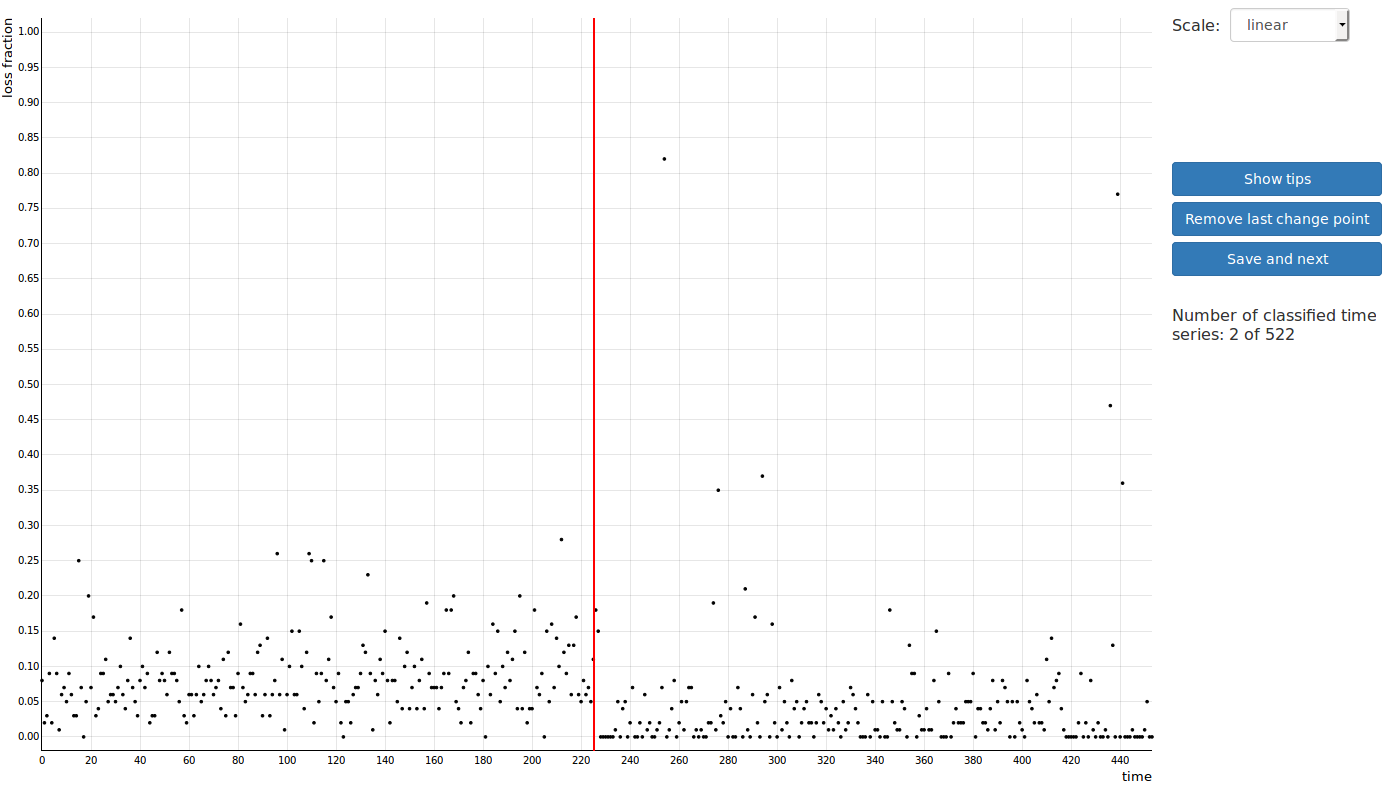
\includegraphics[width=0.9\linewidth]{./figures/methodology/supervised_learning_try/survey_system.png}
    \caption{Survey system snapshot.}
\label{fig:survey_system}
\end{figure}%

X specialists with experience in network measurements and statistical
modeling, but without background in change point detection, classified X time
series.
To analyze the agreement between different users classifications,
for each time series, was applied the Events Times Correlation procedure
described in Section~\ref{sec:events_times_correlation}. Therefore, it was
considered that each user voted to a set of change points positions.
The hours tolerance was set to 7 hours, which means 14 consecutive points. Also
if a user classified points that are too near, it only considered the left most
one. As an example if a user marked a change point at time $t$ and $t + 4$
hours, than it was only considered the point at time $t$.
Then, it
was counted, for each change point voted at least once, the number of
specialists that voted in that change point.
Figure~\ref{fig:classifications_per_vote} shows the histogram of this counting.

\begin{figure}[H]
    \centering
    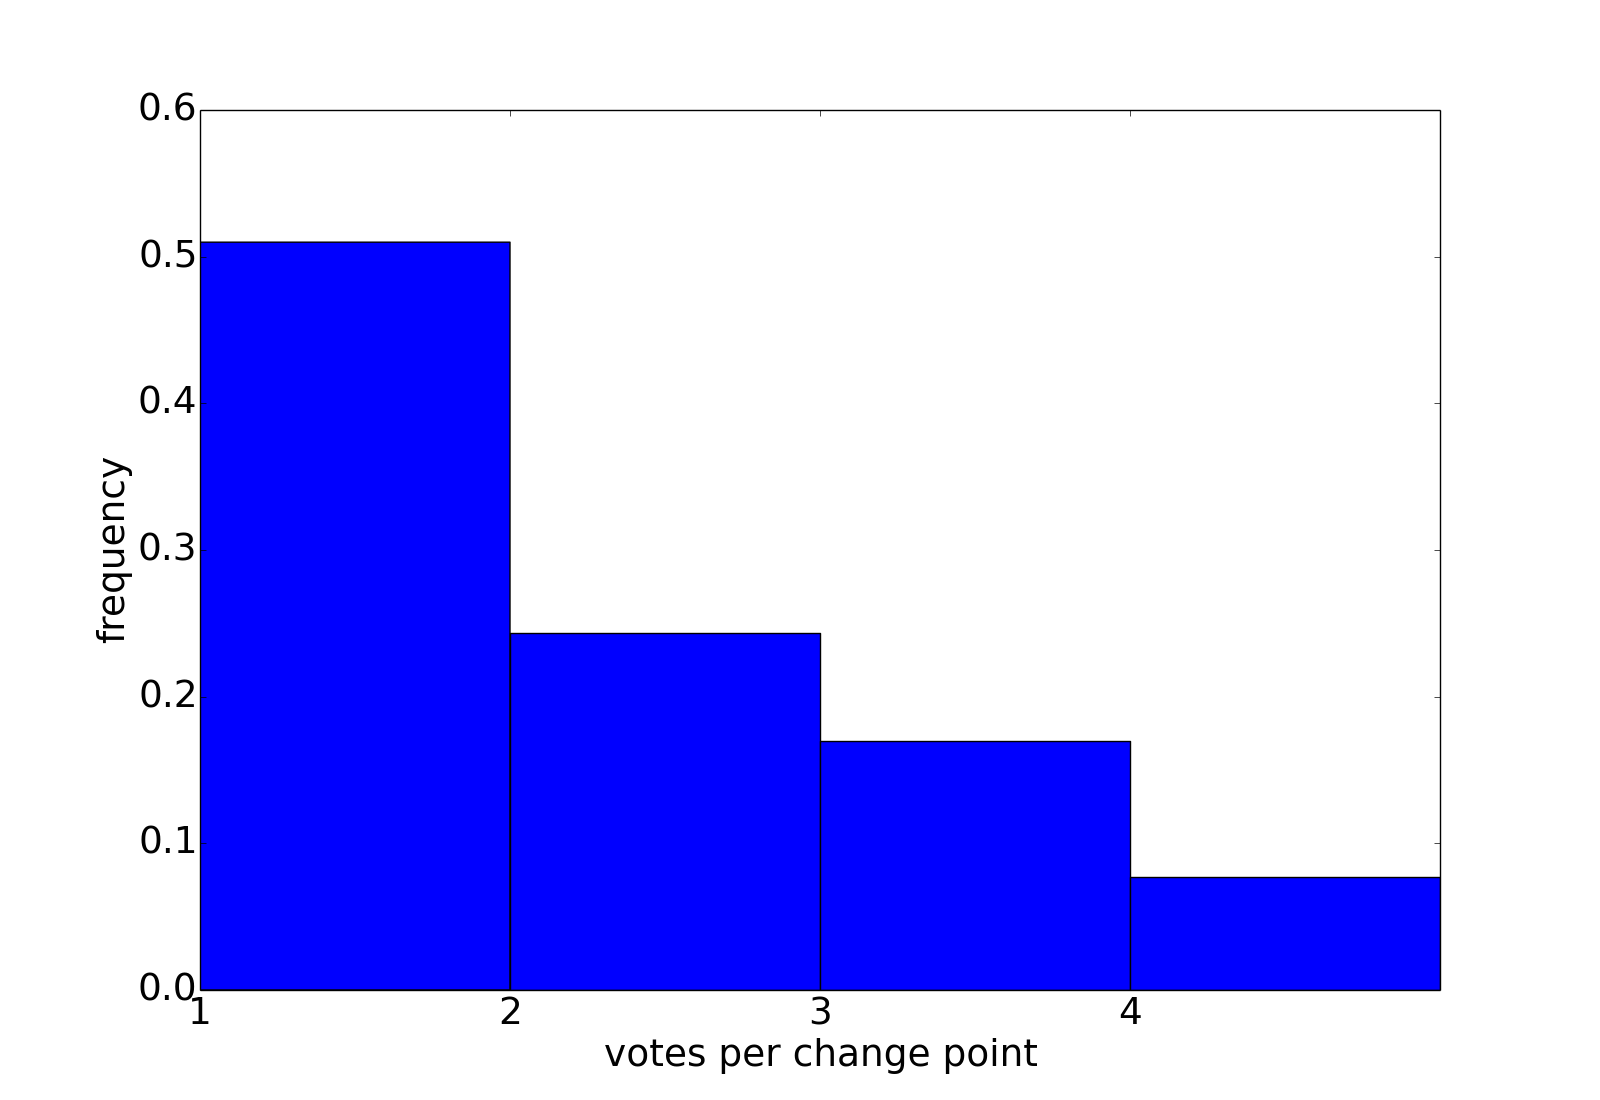
\includegraphics[width=0.9\linewidth]{./figures/methodology/supervised_learning_try/cnt_classifications_per_vote.png}
    \caption{Classifications per vote distribution.}
\label{fig:classifications_per_vote}
\end{figure}%

It is possible to note that, about X\% of the change points were only voted by
a single user, and only Y\% were voted by the majority (more than X votes).
Therefore, in general,
the consesus of change point locations is low.

Next, in Figures~\ref{fig:user_classifications_match} is presented the
classification by users that agree with each other, and
Figure~\ref{fig:user_classifications_unmatch} presents a time series with
several disagreements.

It is possible to note that the users disagrees between them and also that some
users use different statistical classification patterns in the same time
series. At the end of the experiment it was asked to the specialists, and they
sad that their classification pattern changed through they classified time
series, they could classify in different days, and also that the problem is
subjective.

Therefore since, this initial experiment resulted in a noisy dataset, that
probably don't reflect real network events, and that
would be difficult to scale the experiment, including more time series and more
specialists, this strategy was aborted.

However, another result from this experiment is an quantitative study of the
rarity of a
change point. The change point detection problem can be interpreted as a binary
classification problem in which each point of a time series is classified as
``is a change point'' or ``is not a change point''. The voting process, that
resulted in a logical OR opinion of the specialists resulted in X\% of the
points being classfied in change points.

It is important to note that the algorithms presented in
Chapter~\ref{chap:change_point_detection} doesn't use a previous point labels
for a training phase. Once a change point dataset is constructed, in which a
train set each labels each point of a time series as a change point or not, can
open new possibilities to a supervised learning procedure, in which are not
much explored in the literature of change pointe detection.

\section{Differences to Previous Systems}

The high level abstraction of the proposed pipeline has several similarities
with
Argus~\ref{argus_end_to_end_service_anomaly_detection_and_localization_from_an_isps_point_of_view}.
For example, both systems

In general the differences are guided by the data availability and the
measurement process already implemented.

\section{Deployment Issues}
